\documentclass[accentcolor=tud1d,colorbacktitle,inverttitle,landscape,german,presentation,t]{tudbeamer}
\usepackage[latin1]{inputenc}
\usepackage[english]{babel}
\usepackage{amsmath}
\usepackage{amsfonts}
\usepackage{amssymb}
\usepackage{graphicx}
\usepackage{natbib}

\begin{document}
	
	\title[Furuta Pendulum]{Furuta Pendulum - Technical Report}
	\subtitle{Tabea Wilke\\Yannik Frisch\\Maximilian Gehrke \\Group 19 Oleg 
	Arenz}
	
	\author[Tabea Wilke et al.]{Tabea Wilke, Yannik Frisch and Maximilial 
	Gehrke}
	\institute[IAS TU Darmstadt | Group 19]{Institute for Intelligent 
	Autonomous 
	Systems, TU Darmstadt}
	
	
	\logo{
\includegraphics{iasLogo}}
	%\logo{\color{tudtextaccent}\large IFP}
	
	\date{March 22, 2019}
	

\begin{titleframe}
\end{titleframe}
\section{Introduction}
	\begin{frame}
		\frametitle{Introduction}
	
	\begin{minipage}{0.45\textwidth}
		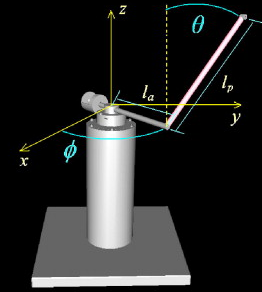
\includegraphics[height=0.9\textheight]{pendulum}
		\cite{la2009new}	
		\end{minipage}
		\begin{minipage}{0.5\textwidth}
			\begin{itemize}
				\item Underactuated System (2 DOF, 1 actuator)
				\item Highly non-linear
				\item Two control problems
				\begin{itemize}
					\item "swing-up"
					\item "stabilization"
				\end{itemize}
			\end{itemize}
		\end{minipage}

	\end{frame}

\section{Control Problems}
\begin{frame}[t]
	\frametitle{Swing-up \& Stabilization}
	\begin{minipage}[t]{0.48\textwidth}
	\textbf{Swing-up}
	\begin{itemize}
		\item Energy control 
		\item Decide whether to "push" or "pull"
	\end{itemize}
	\end{minipage}
\hfill
	\begin{minipage}[t]{0.48\textwidth}
		\textbf{Stabilization}
		\begin{itemize}
		\item Proportional integral derivative (PID)
		\item Linear quadratic regulator (LQR)
		\item Particle swarm, evolutionary algorithms
		\end{itemize}
	\end{minipage}
\end{frame}
\begin{frame}[t]
	\frametitle{Reinforcement Learning on the\\ Furuta Pendulum}
	\begin{itemize}
	\item TD($\lambda$), Kalman filter, Gaussian Process $\rightarrow$ no 
	stabilization
	\item ANN with PID controller $\rightarrow$ only prediction
	\item Our implementations $\rightarrow$ seem to work well
	\end{itemize}
\end{frame}

\begin{frame}[c]
	\frametitle{Summary}
	\begin{itemize}
		\item Complex system
		\item Not yet that relevant in Reinforcement Learning
		\item[ ]
		\item[ ]
		\item[ ] 	\textbf{Can Reinforcement Learning improve results on the 
		Furuta 
		pendulum?}
	\end{itemize}



\end{frame}
\begin{frame}
	\frametitle{Sources}
	\bibliographystyle{dinat}
	\bibliography{furutaPres.bib} 
\end{frame}
\end{document}